\documentclass[../main.tex]{subfiles}
\graphicspath{{\currfiledir}}
\begin{document}
\chapter{Terminology}

\section{Grapheme}
\textcquote[204]{crystal2010}{Graphemes are the smallest units in a writing system capable of 
causing a contrast in meaning.}
In linguistics, graphemes are often placed into angle brackets, e.g. \grapheme{a} or \grapheme{b}.
Sometimes \emph{graphemes} are called \emph{signs}.
The term \emph{sign} and \emph{grapheme} are considered to be equivalent and 
interchangeable throughout this work.

\section{Graph and allograph}
\textcquote[204]{crystal2010}{Graphemes are abstract units which may adopt a variety of forms 
\elide Each of these possible forms is known as \emph{graphs}\elide
There is a vast amount of physical variation in the shapes of graphs that does not affect the 
underlying identity of the grapheme\elide 
When graphs are analyzed as variants of a grapheme, they are known as \emph{allographs}.}
The Maya script uses a lot of allographs.
For example, the syllable \syllable{u} can be written in many ways all having the same meaning.
See~\ref{fig:terminology-grapheme-u-allographs} for a selection of allographs.
\begin{center}
    
\includegraphics[width=\textwidth,keepaspectratio]{img/grapheme-u-allographs}
    \captionof{figure}{Some allographs of the grapheme \grapheme{u}}
    \label{fig:terminology-grapheme-u-allographs}
\end{center}

\section{Hieroglyph and glyph}
The term \emph{hieroglyph} and \emph{glyph} are not precise terms.
Both are used in epigraphic literature, to address a group of one or more graphemes.
\textcquote[1]{bricker1986}{A ``glyph'' is a sign that can occur alone or in combination with 
other signs}.
\textcquote[34]{knorozov1967}{A hieroglyph consists of several graphemes, which are joined 
in writing}. 
Both expressions are considered to be equivalent and interchangeable throughout this work.
\emph{Glyphs} can represent a syllable, a single word or even a whole phrase 
(\cite[23]{macrilooper2003}).

For example, the glyph~\ref{fig:terminology-glyphs-utzapaw} consists of the 
graphemes \grapheme{u}, \grapheme{tz\glottalstop{}a} and \grapheme{wa} representing the phrase
\mayan{u tz\glottalstop{}apaw}, ``she/he erects it''.
The glyph~\ref{fig:terminology-glyphs-ixwinikhaabajaw} consisting of the 
graphemes \grapheme{ix}, \grapheme{winikhaab} and \grapheme{ajaw}
and represents the noble title \mayan{ix winikhaab ajaw}, ``Ruler Lady Winikhaab''.
\begin{figure}
    \centering
    \begin{subfigure}[b]{0.49\textwidth}
        \centering
        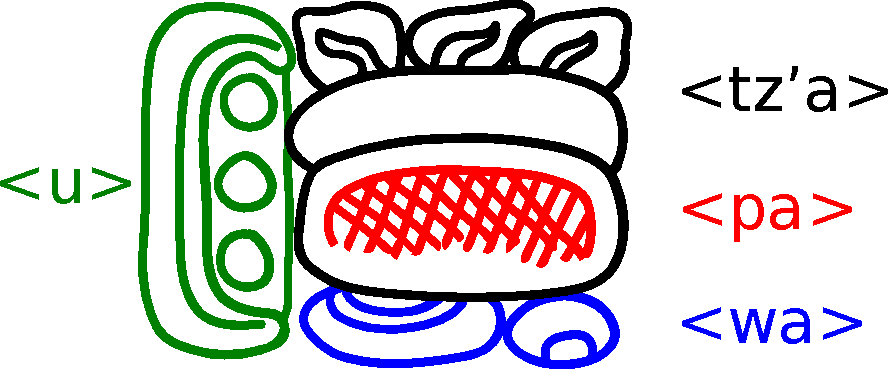
\includegraphics[height=\glyphblockheight]{img/glyphs-utzapaw}
        \caption{\mayan{u tz\glottalstop{}apaw}}
        \label{fig:terminology-glyphs-utzapaw}
    \end{subfigure}
    \hfill
    \begin{subfigure}[b]{0.49\textwidth}
        \centering
        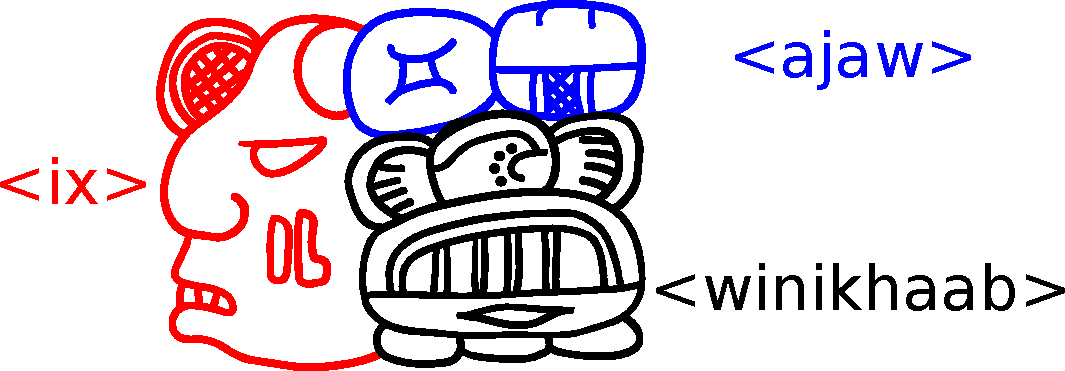
\includegraphics[height=\glyphblockheight]{img/glyphs-ixwinikhaabajaw}
        \caption{\mayan{ix winikhaab ajaw}}
        \label{fig:terminology-glyphs-ixwinikhaabajaw}
    \end{subfigure}
    \caption{Sample glyphs: graphemes are distinguished by different colors}
\end{figure}

\section{Glyph block and collocation}
One or more \emph{Glyphs} are usually arranged in regular rectangular shapes called a 
\emph{glyph block}.
Sometimes they are also called \emph{collocation}.
\textcquote[1]{bricker1986}{A ``collocation'' is a group of signs that occupies a 
defined space, or block, in a hieroglyphic text.}
\textcquote[23]{macrilooper2003}{The rectangular shape of \emph{glyph blocks} results from 
the arrangement of texts into rows and columns}.
\todo{Image/drawing which shows rows and columns of glyphs}

\section{Cataloging of signs}
One of the first steps to analyze an unknown writing system, is to identify distinctive graphemes 
and their allographs. 
In the past, several sign catalogs have been proposed.
Yuri Knorozov created a sign catalog in his work (\cite[109\psq]{knorozov1967}).
William E. Gates' and G\"unter Zimmermann's catalogs (\cite{gates1931}, \cite{zimmermann1956}) are 
based on the Maya codices but did not include the signs from the inscriptions 
(\cite[4]{thompson1962catalog}). 
Eric Thompson extended G\"unter Zimmermann's idea and categorized all signs into affixes, main signs 
(including animal heads) and portrait signs (\cite[4]{thompson1962catalog}).
His catalog covers the Maya codices, the monumental inscriptions and other writings 
(e.g.\ ceramics, vessels, bones).
All catalogs assigned a number to each sign/grapheme.
To distinguish between the different catalog systems, it is common to use a prefix in 
conjunction with the number.
So, for example, all Thompson numbers are labeled with ``T'', e.g. \thompson{510}.

In 2003, Martha J. Macri and Matthew G. Looper proposed a new system which assigns all graphemes
a code consisting of three digits (\cite[21,25]{macrilooper2003}).
The first two digits specifies the category of the sign 
(e.g. A for animals, M for signs with hands etc.) whereas the third digit is an arbitrary number
sequencing the different graphemes.

TODO Mayawoerterbuch (classicmayan.org)


\subsection{Problems and limitations}
Having all these sign catalogs are a huge help to systematically analyze any writing system.
It is especially important when the writing system cannot be read.
As one could see above, researchers assign codes or numbers to address individual or 
even groups of signs.
Therefore, identifying graphemes are crucial to systematically build up a sign catalog.
Yet, determine them in an unknown writing system is challenging.
One way to approach this, is by segmenting the texts into distinct \emph{graphs} .
Researchers hereby followed the assumption that graphemes of a script are considered the same if 
they resemble each other in more features than either resembles any other.
\textcquote[34]{knorozov1967}{Two [signs] are identical when they are both composed of the same 
graphic elements\elide, whose drawing and disposition is sufficiently similar to allow them to 
be identified}.
However, if there is no control in terms of linguistics and content, 
this approach can be problematic.
Three major issues can occur when segmenting signs from an unknown writing system:
\begin{itemize}
    \item Allographs are interpreted as separate graphemes.
    \item Graphemes with distinct phonemes and meanings are interpreted as allographs.
    \item Complex graphemes are split into its sub-graphemic components.
\end{itemize}

Especially in writing systems with many allographs like the Maya hieroglyphs,
allographs are sometimes not recognized and, instead, are interpreted as separate graphemes. 
Another problem is that some signs are considered to be allographs because of their similarities, 
but, as later progress in decipherment has shown, were actually distinct graphemes.
Eric Thompson (\cite[12\psq]{thompson1962catalog}) recognized the method of segmentation as 
a potential source of false conclusions.
David H. Kelley (\cite{kelley1962}) showed in his review of Thompson's sign catalog that
some T-numbers represent more than one grapheme (e.g. TODO) and some 
T-numbers are allographs of another (e.g. TODO).
Despite merging unrelated graphs or separating allographs which actually belong to each other,
the Maya writing system also utilized graphemes which consist of two or more subgraphemic 
components.
Those complex graphemes might not be recognized and therefore only its components are registered
as graphemes.
One of those complex graphemes, is the grapheme \grapheme{pas} ``dawn'' 
(\ref{fig:terminology-glyphs-pas}) which is built from
grapheme \grapheme{chan} ``sky'' (\ref{fig:terminology-glyphs-chan}), 
grapheme \grapheme{k\glottalstop} ``k\glottalstop{}in'' (\ref{fig:terminology-glyphs-kin}) and
grapheme \grapheme{kab} ``earth'' (\ref{fig:terminology-glyphs-kab}).
It can be found, for example, on Tikal Temple IV, Lintel 2 A7.
All three components are graphemes themselves, but in combination they form the complex 
grapheme \grapheme{pas} with its phoneme and meaning.
This grapheme doesn't show up in Thompson's sign catalog.
Later revisions and new catalogs like Macri and Looper (\cite{macrilooper2003}) added it as
separate grapheme and assigned it the code ZX2.
\begin{figure}
    \centering
    \begin{subfigure}[b]{0.24\textwidth}
        \centering
        
\includegraphics[height=\glyphblockheight]{img/grapheme-PAS}
        \caption{\grapheme{pas} ``dawn''}
        \label{fig:terminology-glyphs-pas}
    \end{subfigure}
    \hfill
    \begin{subfigure}[b]{0.24\textwidth}
        \centering
        
\includegraphics[height=\glyphblockheight]{img/grapheme-CHAN}
        \caption{\grapheme{chan} ``sky''}
        \label{fig:terminology-glyphs-chan}
    \end{subfigure}
    \begin{subfigure}[b]{0.24\textwidth}
        \centering
        
\includegraphics[height=\glyphblockheight]{img/grapheme-KIN}
        \caption{\grapheme{k\glottalstop{}in} ``sun''}
        \label{fig:terminology-glyphs-kin}
    \end{subfigure}
    \begin{subfigure}[b]{0.24\textwidth}
        \centering
        
\includegraphics[height=\glyphblockheight]{img/grapheme-KAB}
        \caption{\grapheme{kab} ``earth''}
        \label{fig:terminology-glyphs-kab}
    \end{subfigure}
    \caption{Grapheme \grapheme{pas}. Even though it consists of three other graphemes, 
             it represents a self-contained grapheme with separate phonetic and meaning 
             (\cite[139]{prager2018}).}
\end{figure}

\end{document}
